\newpage
\section{Exercices}
 {
  \small
  \setlength{\columnseprule}{0.6pt}
  \begin{multicols}{2}
	  \begin{exo}[Développement]
		  Développer et réduire les expressions suivantes:
		  \vspace*{-2mm}
		  \begin{multicols}{2}
			  \begin{enumerate}[label=\alph*)]
				  \item $3(x + 2) - 4(2 - 2x)$
				  \item $x(2x - 1) - 3(5 - x)$
				  \item $(3x + 1)x - 3(x - 2)$
				  \item $3(x - 5) - 2x(1 - 2x)$
			  \end{enumerate}
		  \end{multicols}
	  \end{exo}

	  \begin{exo}[Développement]
		  Développer et réduire les expressions suivantes:
		  \begin{enumerate}[label=\alph*)]
			  \item $(2x + 1)(3 - 2x)$
			  \item $(x - 3)(-x - 1)$
			  \item $(3x + 2)(5 - 2x)$
			  \item $(x - 1)(3x^{2} - 2)$
			  \item $(3 - x)(2x + 1) + 2(x + 2)$
			  \item $(x - 1)(2x - 1) - 3(3 + 2x)$
		  \end{enumerate}
	  \end{exo}

	  \begin{exo}[Factorisation]
		  Factoriser et réduire les expressions suivantes :
		  \vspace*{-2mm}
		  \begin{multicols}{2}
			  \begin{enumerate}[label=\alph*)]
				  \item $3x + 6$
				  \item $16x - 4$
				  \item $3x + 9$
				  \item $4x + 6$
				  \item $x^{2} + 3x$
				  \item $7x + 7x^{2}$
				  \item $8x^{2} + 6x$
				  \item $6x + 15x^{2}$
			  \end{enumerate}
		  \end{multicols}
	  \end{exo}

	  \begin{exo}[Factorisation]
		  Factoriser et réduire les expressions suivantes :
		  \begin{enumerate}[label=\alph*)]
			  \item $x(3x + 2) + x(5 - x)$
			  \item $4(5x + 2) + 2x(5x + 2)$
			  \item $(3x + 2)2x + 2x(2 - x)$
			  \item $(1 - 3x)(2 + x) + (1 - 3x)(5 - 2x)$
			  \item $(2x + 3)(4x + 3) - (2x + 3)(x - 1)$
			  \item $(x + 5)(4 - x) - (4 - x)$
			  \item $(x + 1)^{2} + (x + 1)(2x - 3)$
		  \end{enumerate}
	  \end{exo}

	  \begin{exo}[Association d'expressions algébriques]
		  Relier chaque expression de la première colonne avec sa forme développée dans la deuxième colonne.
		  \begin{tabular}{p{3.5cm} @{\hspace{10mm}} p{3cm}}
			  \vspace*{-2mm}
			  \begin{enumerate}[label=\arabic*)]
				  \item $(x + 7)^2$
				  \item $(x + \sqrt{7})^2$
				  \item $(x - 7)(x + 7)$
				  \item $(x^2 + 7)(x^2 - 7)$
				  \item $(x - 7)^2$
			  \end{enumerate}
			   &
			  \vspace*{-2mm}
			  \begin{enumerate}[label=\alph*)]
				  \item $x^2 - 14x + 49$
				  \item $x^2 + 49$
				  \item $x^2 + 14x + 49$
				  \item $x^2 + 7x + 49$
				  \item $x^2 + 2\sqrt{7}x + 7$
				  \item $x^4 - 49$
				  \item $x^2 - 49$
			  \end{enumerate}
			  \\
		  \end{tabular}
	  \end{exo}
	  \vfill~\columnbreak
	  \begin{exo}
		  À l'aide de l'identité remarquable donnée, développer les expressions algébriques suivantes.

		  \def\arraystretch{1.5}
		  \begin{tabular}{m{3.5cm}|m{3.5cm}}
			  $(a + b)^2 = a^2 + 2ab + b^2$ & $(a - b)^2 = a^2 - 2ab + b^2$ \\ \hline
			  \begin{enumerate}[label=\alph*)]
				  \item $(x + 3)^2$
				  \item $(2x + 8)^2$
				  \item $(4 + 3x)^2$
				  \item $\pa{\dfrac{1}{3} + y}^2$
			  \end{enumerate}
			                                &
			  \begin{enumerate}[label=\alph*)]
				  \item $(x - 9)^2$
				  \item $(3x - 4)^2$
				  \item $(2 - 5x)^2$
				  \item $(2y - \sqrt{3})^2$
			  \end{enumerate}
		  \end{tabular}
		  \begin{center}
			  \begin{tabular}{m{3.8cm}}
				  $(a + b)(a - b) = a^2 - b^2$ \\ \hline
				  \begin{enumerate}[label=\alph*)]
					  \item $(x + 14)(x - 14)$
					  \item $(7x + 9)(9 - 7x)$
					  \item $\left( \dfrac{2}{3} + \dfrac{x}{4} \right)\left( \dfrac{2}{3} - \dfrac{x}{4} \right)$
					  \item $\left( z + \dfrac{7}{4} \right)\left( z - \dfrac{35}{20} \right)$
				  \end{enumerate}
			  \end{tabular}
		  \end{center}
	  \end{exo}

	  \begin{exo}
		  À l'aide de l'identité remarquable donnée, factoriser les expressions algébriques suivantes.

		  \def\arraystretch{1.5}
		  \begin{tabular}{m{3.5cm}|m{3.5cm}}
			  $a^2 + 2ab + b^2 = (a + b)^2$ & $a^2 - 2ab + b^2 = (a - b)^2$ \\ \hline
			  \begin{enumerate}[label=\alph*)]
				  \item $x^2 + 10x + 25$
				  \item $9x^2 + 6x + 1$
				  \item $2y + 1 + y^2$
				  \item $4x^2 + 20x + 25$
			  \end{enumerate}
			                                &
			  \begin{enumerate}[label=\alph*)]
				  \item $x^2 - 8x + 16$
				  \item $9x^2 - 6x + 1$
				  \item $z^2 - z + \dfrac{1}{4}$
				  \item $25 + 25x^2 - 50x$
			  \end{enumerate}
		  \end{tabular}

		  \begin{center}
			  \begin{tabular}{m{3.8cm}}
				  $a^2 - b^2 = (a + b)(a - b)$ \\ \hline
				  \begin{enumerate}[label=\alph*)]
					  \item $a^2 - 144$
					  \item $9x^2 - 16$
					  \item $\dfrac{x^2}{4} - \dfrac{4}{9}$
					  \item $x^2 - 7$
				  \end{enumerate}
			  \end{tabular}
		  \end{center}
	  \end{exo}

	  \begin{exo}
		  À l'aide de l'identité remarquable la plus adaptée, développer les expressions algébriques suivantes.
		  \vspace*{-2mm}
		  \begin{multicols}{2}
			  \begin{enumerate}[label=\alph*)]
				  \item $(x + 11)^2$
				  \item $(3x - 7)^2$
				  \item $\left( x - \dfrac{2}{3} \right)\left( x + \dfrac{2}{3} \right)$
				  \item $(5x - 9)(5x + 9)$
				  \item $(2x - 1,5)^2$
				  \item $(x + \sqrt{2})^2$
			  \end{enumerate}
		  \end{multicols}
	  \end{exo}

	  \begin{exo}
		  À l'aide de l'identité remarquable la plus adaptée, factoriser, pour tout nombre réel $x$, les expressions algébriques suivantes.
		  \vspace*{-2mm}
		  \begin{multicols}{2}
			  \begin{enumerate}[label=\alph*)]
				  \item $x^2 + 14x + 49$
				  \item $9x^2 - 30x + 25$
				  \item $x^2 - \dfrac{16}{81}$
				  \item $16x^2 - 4900$
				  \item $6,25 + x^2 - 5x$
				  \item $x^2 + \sqrt{2}x + \dfrac{1}{2}$
			  \end{enumerate}
		  \end{multicols}
	  \end{exo}

	  \vfill~\columnbreak

	  \begin{exo}
		  Dans un plan, on considère une unité de longueur donnée. Soient les deux figures suivantes :

		  \begin{itemize}
			  \item Un rectangle dont les côtés mesurent $\pa{x - 1}$ et $\pa{x + 1}$
			  \item Un carré dont le côté mesure $x$ et dans lequel on a enlevé un carré de $1$ de côté.
		  \end{itemize}

		  \begin{center}
			  \begin{tikzpicture}[scale=0.7,>=Stealth]
				  \draw[very thick] (0,0) rectangle (4,2.5);
				  \draw[<->, thick] (-0.3,0) -- (-0.3,2.5) node[midway, above, sloped] {$x - 1$};
				  \draw[<->, thick] (0,-0.3) -- (4,-0.3) node[midway, below] {$x + 1$};
				  \begin{scope}[shift={(5.5,0)}]
					  \draw[very thick] (0,0) -- (4,0) -- (4,3.5) -- (1,3.5) -- (1,2.5) -- (0,2.5) -- cycle;
					  \draw[<->, thick] (0,2.7) -- (1,2.7) node[midway, above] {$1$};
					  \draw[<->, thick] (0,-0.3) -- (4,-0.3) node[midway, below] {$x$};
				  \end{scope}
			  \end{tikzpicture}
		  \end{center}

		  \begin{enumerate}
			  \item À quel plus grand intervalle $x$ peut-il appartenir ?
			  \item À l'aide d'une calculatrice, calculer l'aire de chacune de ces figures pour différentes valeurs de $x$.
			  \item Que peut-on conjecturer ?
			  \item Montrer que, pour tout $x > 1$, ces deux figures ont la même aire.
		  \end{enumerate}
	  \end{exo}

	  \begin{exo}
		  Dans cet exercice, on cherche à trouver une méthode pour calculer facilement $99^2$.

		  \begin{enumerate}
			  \item Compléter : \cmath{99^2 = (100 - \ldots)^2 = 100^2 - 2 \times \ldots \times \ldots + 1^2 = \ldots}
			  \item En remarquant que $999 = 1000 - 1$ et avec une méthode similaire, calculer $999^2$.
			  \item Avec une méthode similaire, calculer $1001^2$ et $95 \times 105$.
		  \end{enumerate}
	  \end{exo}

	  \begin{exo}
		  On considère l'expression littérale $A(x) = x^2 + 8x + 15$ définie pour tout réel $x$.
		  \begin{enumerate}
			  \item Montrer que $A(x) = (x + 4)^2 - 1$.
			  \item Montrer que $A(x) = (x + 3)(x + 5)$.
			  \item En choisissant la forme de $A(x)$ la plus adaptée à un calcul mental, calculer $A(0)$, $A(-3)$, $A(-4)$ et $A(-5)$.
		  \end{enumerate}
	  \end{exo}

	  \begin{exo}
		  On considère l'expression suivante définie pour tout $x$ : \cmath{B(x) = (4x + 5)^2 - (4x + 5)(7 - x)}

		  \begin{enumerate}
			  \item Pour tout $x$, développer et réduire $B(x)$.
			  \item Pour tout $x$, factoriser $B(x)$ à l'aide d'un facteur commun.
			  \item En déduire la résolution dans $\mathbb{R}$ de \cmath{20x^2 + 17x - 10 = 0}
		  \end{enumerate}
	  \end{exo}

	  \vfill~\columnbreak

	  \begin{exo}[Des cubes ...]
		  Cette figure montre la décomposition en plusieurs solides d'un cube d'arête $a + b$ où $a$ et $b$ sont des nombres réels positifs.

		  \begin{center}
			  \definecolor{cubevert}{RGB}{160,200,30}
			  \definecolor{cubeorange}{RGB}{250,185,40}
			  \definecolor{cubebleu}{RGB}{50,170,200}
			  \definecolor{cuberouge}{RGB}{225,85,35}
			  \newcommand{\boite}[7]{%
				  {\pgfmathsetmacro{\xb}{#1+#4}%
						  \pgfmathsetmacro{\yb}{#2+#5}%
						  \pgfmathsetmacro{\zb}{#3+#6}%
						  \filldraw[fill=#7!70!white, draw=white, line join=round, line width=0.4pt]
						  (#1,#2,\zb) -- (\xb,#2,\zb) -- (\xb,\yb,\zb) -- (#1,\yb,\zb) -- cycle;
						  \filldraw[fill=#7, draw=white, line join=round, line width=0.4pt]
						  (\xb,#2,#3) -- (\xb,\yb,#3) -- (\xb,\yb,\zb) -- (\xb,#2,\zb) -- cycle;
						  \filldraw[fill=#7!75!black, draw=white, line join=round, line width=0.4pt]
						  (#1,\yb,#3) -- (\xb,\yb,#3) -- (\xb,\yb,\zb) -- (#1,\yb,\zb) -- cycle;}%
			  }

			  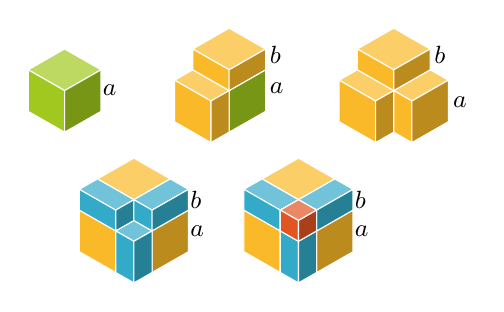
\begin{tikzpicture}[scale=1.1, x={(-0.21cm,-0.12cm)}, y={(0.21cm,-0.12cm)}, z={(0cm,0.24cm)}, font=\small]
				  \begin{scope}
					  \boite{0}{0}{0}{2}{2}{2}{cubevert}
					  \node[right=-1mm] at (0,2,1) {$a$};
				  \end{scope}
				  \begin{scope}[xshift=1.9cm]
					  \boite{0}{0}{0}{2}{2}{2}{cubevert}
					  \boite{2}{0}{0}{1}{2}{2}{cubeorange}
					  \boite{0}{0}{2}{2}{2}{1}{cubeorange}
					  \node[right=-3mm] at (0,3,3.2) {$b$};
					  \node[right=-3mm] at (0,3,1.6) {$a$};
				  \end{scope}
				  \begin{scope}[xshift=3.8cm]
					  \boite{2}{0}{0}{1}{2}{2}{cubeorange}
					  \boite{0}{2}{0}{2}{1}{2}{cubeorange}
					  \boite{0}{0}{2}{2}{2}{1}{cubeorange}
					  \node[right=-3mm] at (0,3,3.2) {$b$};
					  \node[right=1mm] at (0,2.3,0.6) {$a$};
				  \end{scope}
				  \begin{scope}[xshift=0.8cm, yshift=-1.5cm]
					  \boite{2}{0}{0}{1}{2}{2}{cubeorange}
					  \boite{0}{2}{0}{2}{1}{2}{cubeorange}
					  \boite{0}{0}{2}{2}{2}{1}{cubeorange}
					  \boite{2}{2}{0}{1}{1}{2}{cubebleu}
					  \boite{2}{0}{2}{1}{2}{1}{cubebleu}
					  \boite{0}{2}{2}{2}{1}{1}{cubebleu}
					  \node[right=-1mm] at (0,3,2.5) {$b$};
					  \node[right=-1mm] at (0,3,1)   {$a$};
				  \end{scope}
				  \begin{scope}[xshift=2.7cm,yshift=-1.5cm]
					  \boite{2}{0}{0}{1}{2}{2}{cubeorange}
					  \boite{0}{2}{0}{2}{1}{2}{cubeorange}
					  \boite{0}{0}{2}{2}{2}{1}{cubeorange}
					  \boite{2}{2}{0}{1}{1}{2}{cubebleu}
					  \boite{2}{0}{2}{1}{2}{1}{cubebleu}
					  \boite{0}{2}{2}{2}{1}{1}{cubebleu}
					  \boite{2}{2}{2}{1}{1}{1}{cuberouge}
					  \node[right=-1mm] at (0,3,2.5) {$b$};
					  \node[right=-1mm] at (0,3,1)   {$a$};
				  \end{scope}
			  \end{tikzpicture}
		  \end{center}

		  \begin{enumerate}
			  \item Pour chaque couleur de solide (vert, jaune, bleu et rouge) :
			        \begin{enumerate}
				        \item Déterminer le nombre de solides.
				        \item Déterminer le volume d'un solide en fonction de $a$ et $b$.
			        \end{enumerate}
			  \item Montrer que $(a + b)^3 = a^3 + 3a^2b + 3ab^2 + b^3$.
			  \item Cette égalité est-elle démontrée pour tous $a$ et $b$ ?
		  \end{enumerate}
	  \end{exo}

	  \begin{exo}[... et des carrés]
		  On considère le carré $ABCD$ de côtés $6\text{ cm}$ et quatre points $M$, $N$, $P$, $Q$ tels que $AM = BN = CP = DQ$

		  On admet que $MNPQ$ est un carré et on note $x = BM$

		  \begin{center}
			  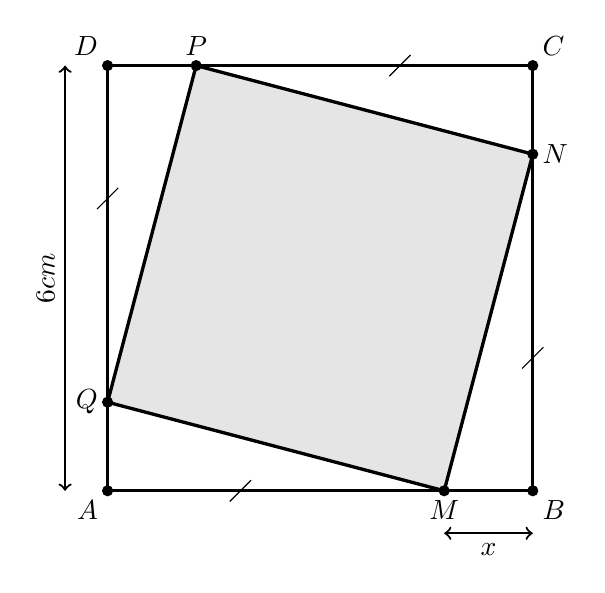
\begin{tikzpicture}[scale=0.9]
				  \coordinate (A) at (0,0);
				  \coordinate (B) at (6,0);
				  \coordinate (C) at (6,6);
				  \coordinate (D) at (0,6);
				  \draw[very thick] (A) -- (B) -- (C) -- (D) -- cycle;
				  \node[below left] at (A) {$A$};
				  \node[below right] at (B) {$B$};
				  \node[above right] at (C) {$C$};
				  \node[above left] at (D) {$D$};
				  \coordinate (M) at (4.75,0);
				  \coordinate (N) at (6,4.75);
				  \coordinate (P) at (1.25,6);
				  \coordinate (Q) at (0,1.25);
				  \draw[very thick, fill=black!10] (M) -- (N) -- (P) -- (Q) -- cycle;
				  \node[below] at (M) {$M$};
				  \node[right] at (N) {$N$};
				  \node[above] at (P) {$P$};
				  \node[left] at (Q) {$Q$};
				  \draw[<->, thick] (-0.6,0) -- (-0.6,6) node[midway, above, sloped] {$6\text{ cm}$};
				  \draw[<->, thick] (4.75,-0.6) -- (6,-0.6) node[midway, below] {$x$};
				  \draw[shift={(1.875,0)}] (-0.15,-0.15) -- (0.15,0.15);
				  \draw[shift={(6,1.875)}] (-0.15,-0.15) -- (0.15,0.15);
				  \draw[shift={(4.125,6)}] (-0.15,-0.15) -- (0.15,0.15);
				  \draw[shift={(0,4.125)}] (-0.15,-0.15) -- (0.15,0.15);
				  \foreach \pt in {A,B,C,D,M,N,P,Q} { \filldraw[black] (\pt) circle (2pt); }
			  \end{tikzpicture}
		  \end{center}

		  \begin{enumerate}
			  \item Justifier que l'aire $\mathcal{A}$ du carré $MNPQ$ a pour valeur : \cmath{\mathcal{A} = 2x^2 - 12x + 36}
		  \end{enumerate}

		  \textbf{Aide :} $\text{Aire}(MNPQ) = \text{Aire}(ABCD) - 4 \times \text{Aire}(AMQ)$

		  \begin{enumerate}[resume]
			  \item \begin{enumerate}
				        \item Montrer que : \cmath{2(x - 2)(x - 4)\ =\ 2x^2 - 12x + 16}
				        \item Déterminer la ou les valeurs de $x$ afin que l'aire du carré $MNPQ$ soit égale aux $\dfrac{5}{9}$ de celle du carré $ABCD$.
			        \end{enumerate}
		  \end{enumerate}
	  \end{exo}

	  \vfill~
  \end{multicols}
 }
